% nouez architecture and message reference.
% Build: pdflatex architecture.tex (twice, for the table of contents).
\documentclass[10pt,a4paper]{article}

\usepackage[margin=2cm]{geometry}
\usepackage[T1]{fontenc}
\usepackage{lmodern}
\usepackage{microtype}
\usepackage{xcolor}
\usepackage{tikz}
\usetikzlibrary{arrows.meta,positioning,fit,backgrounds,calc}
\usepackage{listings}
\usepackage{booktabs}
\usepackage{tabularx}
\usepackage{array}
\usepackage{enumitem}
\usepackage{caption}
\usepackage{float}
\usepackage[hidelinks]{hyperref}

\setlist{nosep,leftmargin=1.5em}
\setlength{\parskip}{0.4em}
\setlength{\parindent}{0pt}

% --- colours -----------------------------------------------------------------
\definecolor{cc}{HTML}{D97757}      % Claude Code
\definecolor{nz}{HTML}{3B6EA8}      % nouez
\definecolor{cx}{HTML}{2E8B57}      % Codex
\definecolor{os}{HTML}{7A6A9E}      % operating system
\definecolor{codebg}{HTML}{F6F7F9}
\definecolor{codeframe}{HTML}{D5D9E0}
\definecolor{str}{HTML}{A33A3A}
\definecolor{muted}{HTML}{6B7280}

% --- code listings -------------------------------------------------------------
\lstdefinestyle{boxed}{
  basicstyle=\ttfamily\scriptsize,
  backgroundcolor=\color{codebg},
  frame=single, rulecolor=\color{codeframe}, framesep=4pt,
  breaklines=true, breakatwhitespace=false, columns=fullflexible,
  keepspaces=true, showstringspaces=false,
  aboveskip=0.5em, belowskip=0.6em,
  captionpos=t,
}
\lstdefinestyle{wire}{style=boxed, stringstyle=\color{str}, morestring=[b]"}
% keep a listing's title with its first lines: break here only if under 6 lines remain
\newcommand{\keeptitle}{\par\vskip 0pt plus 6\baselineskip\penalty-200\vskip 0pt plus -6\baselineskip}
% JSON on the wire: strings coloured
\lstnewenvironment{wire}[1][]{\keeptitle\lstset{style=wire,title={\footnotesize\sffamily #1}}}{}
% plain text (tool results, commands): no string colouring
\lstnewenvironment{plain}[1][]{\keeptitle\lstset{style=boxed,title={\footnotesize\sffamily #1}}}{}

% --- diagram styles --------------------------------------------------------------
\tikzset{
  box/.style={draw, rounded corners=3pt, thick, align=center, inner sep=6pt, font=\small\sffamily},
  actor/.style={box, minimum width=2.6cm, fill=white, font=\footnotesize\sffamily\bfseries},
  lifeline/.style={dotted, gray!45},
  call/.style={-{Stealth[length=2.2mm]}, thick},
  reply/.style={-{Stealth[length=2.2mm]}, densely dashed},
  lbl/.style={font=\scriptsize\ttfamily, inner sep=1pt},
  note/.style={font=\scriptsize\sffamily\itshape, text=muted, align=left},
  edge/.style={-{Stealth[length=2.5mm]}, very thick},
  biedge/.style={{Stealth[length=2.5mm]}-{Stealth[length=2.5mm]}, very thick},
}

% Sequence-diagram helpers. Lifelines are placed at x positions given in cm.
% \lifelines{x/Name/colour, ...}{depth}
\newcommand{\lifelines}[2]{%
  \foreach \x/\name/\col in {#1} {%
    \node[actor, draw=\col, text=\col] at (\x,0) {\name};
    \draw[lifeline] (\x,-0.4) -- (\x,-#2);
  }}
% \msg{y}{from x}{to x}{label}   solid call
\newcommand{\msg}[4]{\draw[call] (#2,-#1) -- node[above=1pt,lbl]{#4} (#3,-#1);}
% \ret{y}{from x}{to x}{label}   dashed reply
\newcommand{\ret}[4]{\draw[reply] (#2,-#1) -- node[above=1pt,lbl]{#4} (#3,-#1);}
% \side{y}{x}{text}               note to the right of a lifeline
\newcommand{\side}[3]{\node[note, anchor=west] at (#2+0.15,-#1) {#3};}
% \frm{y top}{y bottom}{x left}{x right}{label}   a loop / alt frame
\newcommand{\frm}[5]{%
  \draw[gray, rounded corners=2pt] (#3,-#1) rectangle (#4,-#2);
  \node[anchor=north west, font=\scriptsize\sffamily\bfseries, text=gray, fill=white, inner sep=2pt] at (#3,-#1) {#5};}

\newcommand{\code}[1]{\texttt{#1}}
\newcommand{\ccname}{\textcolor{cc}{\textbf{Claude Code}}}
\newcommand{\nzname}{\textcolor{nz}{\textbf{nouez}}}
\newcommand{\cxname}{\textcolor{cx}{\textbf{Codex}}}

\title{\textbf{nouez} 0.4.0\\[0.3em]\large Architecture and message reference}
\date{October 9, 2026}
\author{}

\begin{document}
\maketitle
\vspace{-2em}

\begin{abstract}
\noindent nouez is an MCP server that lets Claude Code consult live Codex sessions. This document
describes nouez 0.4.0: how the pieces fit together, and an example of every message nouez sends
or acts on at each boundary: the MCP traffic between Claude Code and nouez, the WebSocket
JSON-RPC traffic between nouez and the Codex app-server daemon, and the commands nouez runs on
the operating system. The daemon also sends notifications and its own requests, which nouez
discards and this document leaves out. Message shapes are as captured in runs with Claude Code
2.1.295 and Codex app-server daemon 0.162.0; client behaviour described here (the discovery
probe, progress tokens, the 120-second move to the background) was observed in those runs and is
not something nouez controls. Ids are invented, long objects are trimmed to the fields nouez
reads, and quoted error texts marked as excerpts are shortened.
\end{abstract}

\tableofcontents
\newpage

% =============================================================================
\section{Overview}

Two coding agents look at a problem differently. nouez gives each a fixed role:
\ccname{} is the main developer and owns the work; \cxname{} is a consultant that Claude asks
for second opinions. Consultants that nouez starts run in a read-only sandbox, and
\code{StartConsultant} only ever reuses those. Claude can also message a Codex session the user
opened, by name and with \code{allow\_user\_session: true}, when the user asks; such a session
keeps the user's own permissions. Everything
happens from the single Claude Code terminal.

A message makes three hops (Figure~\ref{fig:components}):

\begin{enumerate}
  \item \textbf{Claude Code $\leftrightarrow$ nouez.} Claude Code starts \code{server.py} as a child
        process and speaks MCP to it: JSON-RPC~2.0, one JSON object per line on stdin/stdout.
  \item \textbf{nouez $\leftrightarrow$ Codex daemon.} A tool call that needs the daemon starts
        \code{codex app-server proxy} (usually once per call; WatchConsultant may connect twice),
        which relays its stdio to the daemon's local control socket.
        Over that pipe nouez performs a WebSocket handshake and then exchanges JSON-RPC messages
        in WebSocket text frames.
  \item \textbf{nouez $\rightarrow$ operating system.} To show a consultant to the user, nouez opens a
        terminal pane running \code{codex resume <id>}, which attaches to the same daemon
        session. It also checks for such panes and, on StopConsultant, tries to close them.
\end{enumerate}

\begin{figure}[H]
\centering
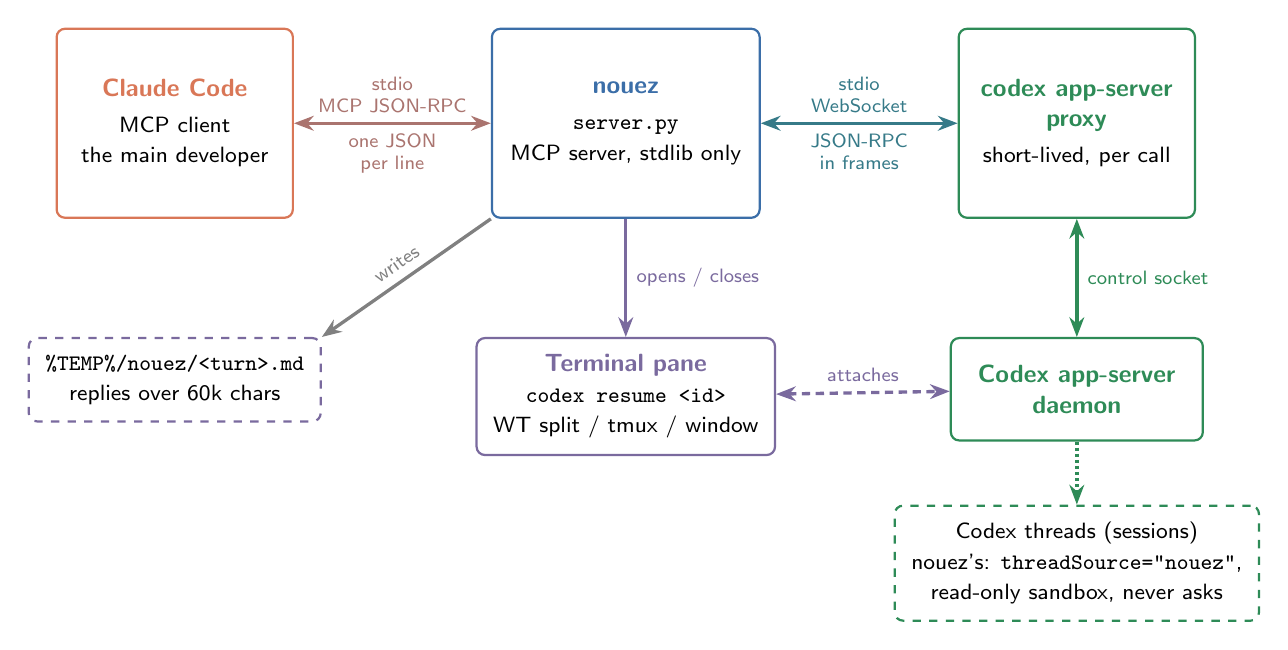
\begin{tikzpicture}[node distance=1.2cm]
  \node[box, draw=cc, minimum width=3.0cm, minimum height=2.4cm] (cc) {\textcolor{cc}{\textbf{Claude Code}}\\[2pt]\footnotesize MCP client\\\footnotesize the main developer};
  \node[box, draw=nz, minimum width=3.4cm, minimum height=2.4cm, right=2.5cm of cc] (nz) {\textcolor{nz}{\textbf{nouez}}\\[2pt]\footnotesize \code{server.py}\\\footnotesize MCP server, stdlib only};
  \node[box, draw=cx, minimum width=3.0cm, minimum height=2.4cm, right=2.5cm of nz] (px) {\textcolor{cx}{\textbf{codex app-server}}\\\textcolor{cx}{\textbf{proxy}}\\[2pt]\footnotesize short-lived, per call};
  \node[box, draw=cx, minimum width=3.2cm, minimum height=1.3cm, below=1.5cm of px] (dm) {\textcolor{cx}{\textbf{Codex app-server}}\\\textcolor{cx}{\textbf{daemon}}};
  \node[box, draw=cx, dashed, minimum width=3.2cm, below=0.8cm of dm] (th) {\footnotesize Codex threads (sessions)\\\footnotesize nouez's: \code{threadSource="nouez"},\\\footnotesize read-only sandbox, never asks};
  \node[box, draw=os, minimum width=3.6cm, below=1.5cm of nz] (term) {\textcolor{os}{\textbf{Terminal pane}}\\\footnotesize \code{codex resume <id>}\\\footnotesize WT split / tmux / window};
  \node[box, draw=os, dashed, minimum width=3.2cm, below=1.5cm of cc] (tmp) {\footnotesize \code{\%TEMP\%/nouez/<turn>.md}\\\footnotesize replies over 60k chars};

  \draw[biedge, cc!70!nz] (cc) -- node[above, font=\scriptsize\sffamily, align=center]{stdio\\MCP JSON-RPC} node[below, font=\scriptsize\sffamily, align=center]{one JSON\\per line} (nz);
  \draw[biedge, nz!60!cx] (nz) -- node[above, font=\scriptsize\sffamily, align=center]{stdio\\WebSocket} node[below, font=\scriptsize\sffamily, align=center]{JSON-RPC\\in frames} (px);
  \draw[biedge, cx] (px) -- node[right, font=\scriptsize\sffamily]{control socket} (dm);
  \draw[edge, cx, densely dotted] (dm) -- (th);
  \draw[edge, os] (nz) -- node[right, font=\scriptsize\sffamily]{opens / closes} (term);
  \draw[biedge, os, densely dashed] (term) -- node[above, font=\scriptsize\sffamily]{attaches} (dm);
  \draw[edge, gray] (nz.south west) -- node[above, sloped, font=\scriptsize\sffamily]{writes} (tmp.north east);
\end{tikzpicture}
\caption{Components and links. Solid arrows carry messages; the terminal pane and nouez share a
Codex session through the daemon, not through each other.}
\label{fig:components}
\end{figure}

\begin{table}[h]
\centering\small
\begin{tabularx}{\textwidth}{@{}l X X X@{}}
\toprule
 & \textbf{Claude Code $\leftrightarrow$ nouez} & \textbf{nouez $\leftrightarrow$ Codex daemon} & \textbf{nouez $\rightarrow$ OS} \\
\midrule
Lifetime & whole Claude Code session & short-lived, opened by the tool call & per command \\
Transport & stdin/stdout of \code{server.py} & stdio of \code{codex app-server proxy} & child processes \\
Framing & newline-delimited JSON & WebSocket frames (RFC 6455) & argv / exit code / stdout \\
Protocol & MCP (JSON-RPC 2.0) & Codex app-server JSON-RPC (no \code{"jsonrpc"} field) & \code{wt}, \code{tmux}, \code{osascript}, PowerShell, \code{pgrep} \\
Who asks & mostly Claude Code; nouez asks \code{roots/list} & nouez (daemon requests are discarded) & always nouez \\
Section & \ref{sec:mcp} & \ref{sec:codex} & \ref{sec:os} \\
\bottomrule
\end{tabularx}
\caption{The three interfaces.}
\end{table}

% =============================================================================
\section{Inside the server}
\label{sec:inside}

\code{server.py} is a single file using only the Python standard library. One thread reads
stdin; every request runs on its own worker thread, because a tool call can block for minutes
while Codex works.

\begin{figure}[H]
\centering
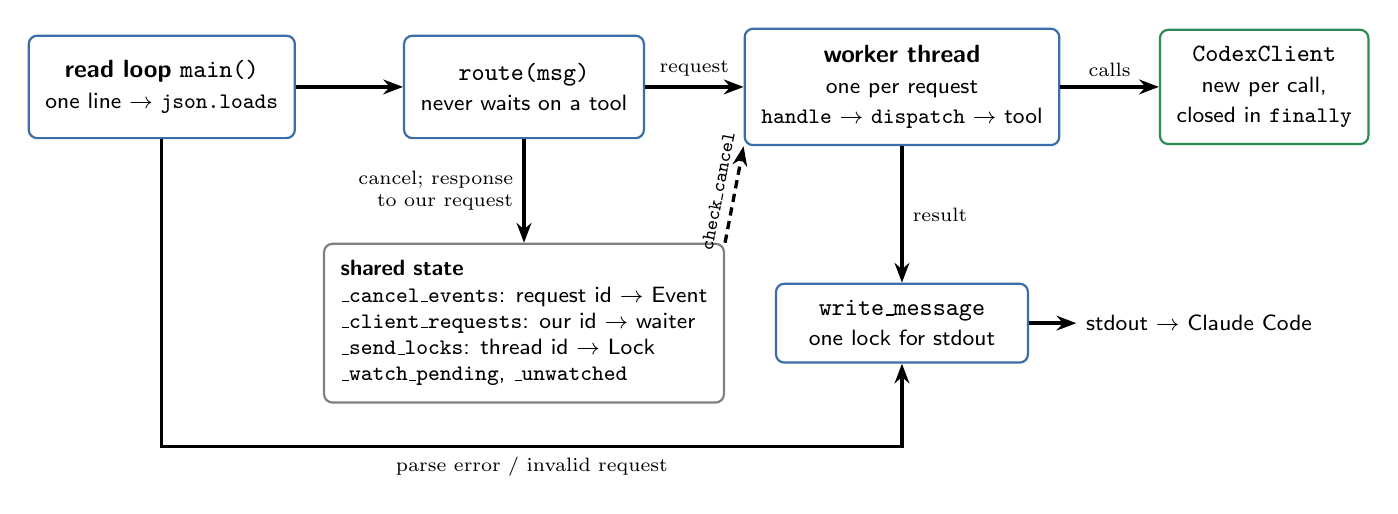
\begin{tikzpicture}[font=\small\sffamily]
  \node[box, draw=nz, minimum width=3.0cm, minimum height=1.3cm] (loop) at (0,0) {\textbf{read loop} \code{main()}\\\footnotesize one line $\rightarrow$ \code{json.loads}};
  \node[box, draw=nz, minimum width=2.6cm, minimum height=1.3cm] (route) at (4.6,0) {\textbf{\code{route(msg)}}\\\footnotesize never waits on a tool};
  \node[box, draw=nz, minimum width=3.2cm, minimum height=1.3cm] (work) at (9.4,0) {\textbf{worker thread}\\\footnotesize one per request\\\footnotesize \code{handle} $\rightarrow$ \code{dispatch} $\rightarrow$ tool};
  \node[box, draw=cx, minimum width=2.6cm, minimum height=1.3cm] (cx) at (14.0,0) {\textbf{\code{CodexClient}}\\\footnotesize new per call,\\\footnotesize closed in \code{finally}};
  \node[box, draw=gray, align=left, font=\footnotesize\sffamily] (reg) at (4.6,-3.0) {\textbf{shared state}\\
    \code{\_cancel\_events}: request id $\rightarrow$ Event\\
    \code{\_client\_requests}: our id $\rightarrow$ waiter\\
    \code{\_send\_locks}: thread id $\rightarrow$ Lock\\
    \code{\_watch\_pending}, \code{\_unwatched}};
  \node[box, draw=nz, minimum width=3.2cm] (out) at (9.4,-3.0) {\textbf{\code{write\_message}}\\\footnotesize one lock for stdout};
  \node[font=\footnotesize\sffamily, right=0.6cm of out] (stdout) {stdout $\rightarrow$ Claude Code};

  \draw[edge] (loop) -- (route);
  \draw[edge] (route) -- node[above, font=\scriptsize]{request} (work);
  \draw[edge] (work) -- node[above, font=\scriptsize]{calls} (cx);
  \draw[edge] (route) -- node[left, font=\scriptsize, align=right]{cancel; response\\to our request} (reg);
  \draw[edge, densely dashed] (reg.north east) -- node[above, sloped, font=\scriptsize]{\code{check\_cancel}} (work.south west);
  \draw[edge] (work) -- node[right, font=\scriptsize]{result} (out);
  \draw[edge] (out) -- (stdout);
  \draw[edge] (loop.south) -- ++(0,-3.9) -| node[pos=0.25, below, font=\scriptsize]{parse error / invalid request} (out.south);
\end{tikzpicture}
\caption{Threading model. Only \code{write\_message} touches stdout, and logs go to stderr, so
stdout carries nothing but MCP messages.}
\end{figure}

\code{route()} sorts each parsed line:

\begin{itemize}
  \item Not an object, an \code{id} that isn't a string or number (booleans included), or a
        request with \code{"id": null}: answer \code{-32600 Invalid Request} right away, from the
        read loop's thread.
  \item No \code{method}: it is Claude Code's answer to a request nouez sent (\code{roots/list}); wake the waiting thread. Answers nobody is waiting for are dropped.
  \item \code{notifications/cancelled}: set the Event of the named request, if it is still running. Malformed params are ignored.
  \item Anything else: register a cancel Event for \code{tools/call} before starting its worker
        thread, so a cancel that arrives while the worker starts up is not lost. (A cancel that
        arrives before its request has nothing to cancel and is ignored.)
\end{itemize}

Any exception inside \code{route()} is logged and the loop continues, so no single line can stop
the server. Inside the worker, \code{handle()} makes sure every request with an id gets a
response unless it was cancelled: if \code{dispatch()} raises, it answers
\code{-32603 Internal error: <exception>}. An exception inside a tool is different: it becomes an
\code{isError} result reading \emph{``Unexpected error: <exception>''}.

% =============================================================================
\section{Claude Code \texorpdfstring{$\leftrightarrow$}{<->} nouez (MCP)}
\label{sec:mcp}

\subsection{Startup}

Claude Code 2.1.295 first probes the 2026-07-28 protocol with \code{server/discover}. nouez is a
legacy-lifecycle server, so it answers \code{-32601}, and Claude Code falls back to the
\code{initialize} handshake with protocol 2025-11-25.

\begin{figure}[H]
\centering
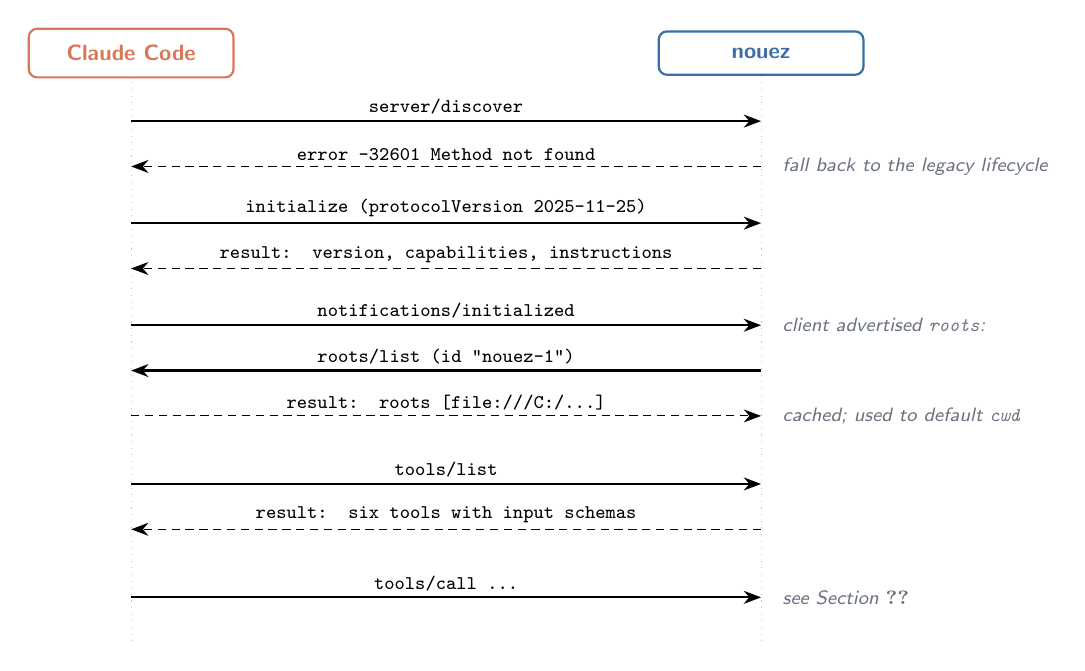
\begin{tikzpicture}[x=1cm,y=0.72cm]
  \lifelines{0/Claude Code/cc, 8/nouez/nz}{10.4}
  \msg{1.2}{0}{8}{server/discover}
  \ret{2.0}{8}{0}{error -32601 Method not found}
  \side{2.0}{8}{fall back to the legacy lifecycle}
  \msg{3.0}{0}{8}{initialize (protocolVersion 2025-11-25)}
  \ret{3.8}{8}{0}{result: version, capabilities, instructions}
  \msg{4.8}{0}{8}{notifications/initialized}
  \side{4.8}{8}{client advertised \code{roots}:}
  \msg{5.6}{8}{0}{roots/list (id "nouez-1")}
  \ret{6.4}{0}{8}{result: roots [file:///C:/...]}
  \side{6.4}{8}{cached; used to default \code{cwd}}
  \msg{7.6}{0}{8}{tools/list}
  \ret{8.4}{8}{0}{result: six tools with input schemas}
  \msg{9.6}{0}{8}{tools/call ...}
  \side{9.6}{8}{see Section~\ref{sec:tools}}
\end{tikzpicture}
\caption{MCP startup.}
\end{figure}

\begin{wire}[Claude Code $\rightarrow$ nouez: discovery probe]
{"jsonrpc": "2.0", "id": 0, "method": "server/discover", "params": {}}
\end{wire}
\begin{wire}[nouez $\rightarrow$ Claude Code]
{"jsonrpc": "2.0", "id": 0, "error": {"code": -32601, "message": "Method not found: server/discover"}}
\end{wire}

\begin{wire}[Claude Code $\rightarrow$ nouez: initialize]
{"jsonrpc": "2.0", "id": 1, "method": "initialize", "params": {
  "protocolVersion": "2025-11-25",
  "capabilities": {"roots": {"listChanged": true}, "elicitation": {"form": {}, "url": {}}},
  "clientInfo": {"name": "claude-code", "version": "2.1.295"}}}
\end{wire}

nouez answers with the requested version if it supports it (2025-11-25, 2025-06-18 or
2025-03-26) and with 2025-11-25 otherwise. It never echoes an unknown version.

\begin{wire}[nouez $\rightarrow$ Claude Code]
{"jsonrpc": "2.0", "id": 1, "result": {
  "protocolVersion": "2025-11-25",
  "capabilities": {"tools": {}},
  "serverInfo": {"name": "nouez", "version": "0.4.0"},
  "instructions": "Whenever the user asks for a Codex consultant, call StartConsultant with cwd set to your working directory, even if you don't remember one being open (earlier context may have been compacted). It reuses a consultant it started earlier in this repo, ... A result that says 'still working' is not a reply, even if it shows output so far: call GetConsultantReply with wait=\"done\" again rather than treating it as done."}}
\end{wire}

\begin{wire}[Claude Code $\rightarrow$ nouez]
{"jsonrpc": "2.0", "method": "notifications/initialized"}
\end{wire}

Because Claude Code advertised \code{roots}, nouez asks for its workspace folders. It does this on
a worker thread and waits at most 5 seconds; a client that never answers counts as having no
roots. The same request is sent again on \code{notifications/roots/list\_changed}.

\begin{wire}[nouez $\rightarrow$ Claude Code: server-initiated request]
{"jsonrpc": "2.0", "id": "nouez-1", "method": "roots/list", "params": {}}
\end{wire}
\begin{wire}[Claude Code $\rightarrow$ nouez]
{"jsonrpc": "2.0", "id": "nouez-1", "result": {"roots": [
  {"uri": "file:///C:/Users/you/Projects/nouez", "name": "nouez"}]}}
\end{wire}

\begin{wire}[Claude Code $\rightarrow$ nouez]
{"jsonrpc": "2.0", "id": 2, "method": "tools/list", "params": {}}
\end{wire}
\begin{wire}[nouez $\rightarrow$ Claude Code (one of six tools shown)]
{"jsonrpc": "2.0", "id": 2, "result": {"tools": [
  {"name": "SendConsultantMessage",
   "description": "Send a message into a Codex session and, by default, wait for and return its reply. ...",
   "inputSchema": {"type": "object",
     "properties": {
       "to": {"type": "string", "description": "Consultant name, thread id, or unique id prefix/suffix."},
       "message": {"type": "string", "description": "The message to send."},
       "from": {"type": "string", "description": "Sender label shown to Codex, ..."},
       "wait": {"anyOf": [{"type": "number", "minimum": 0, "maximum": 14400},
                          {"type": "string", "enum": ["done"]}],
                "description": "How long to wait for the reply: a number of seconds (0 = don't wait), or \"done\" ... Default 600. ..."},
       "allow_user_session": {"type": "boolean", "description": "Allow sending to a Codex session the user opened ... Default false. ..."}},
     "required": ["to", "message"]},
   "annotations": {"readOnlyHint": false, "destructiveHint": false}},
  ...]}}
\end{wire}

Each tool carries annotations, hints a client may use when deciding what to confirm:

\begin{center}\small
\begin{tabular}{@{}l l l l@{}}
\toprule
\textbf{Tool} & \code{readOnlyHint} & \code{destructiveHint} & \textbf{also} \\
\midrule
StartConsultant & false & false & \\
ListConsultants & true & & \code{openWorldHint: false} \\
SendConsultantMessage & false & false & \\
GetConsultantReply & true$^*$ & & \code{openWorldHint: false} \\
WatchConsultant & false & false & \code{idempotentHint: true}, \code{openWorldHint: false} \\
StopConsultant & false & true & \code{openWorldHint: false} \\
\bottomrule
\end{tabular}
\end{center}

{\small $^*$Its only write is nouez's own copy of an over-long reply in the temp folder
(Section~\ref{sec:send}).}

\code{ping} is answered with an empty result: \code{\{"jsonrpc": "2.0", "id": 9, "result": \{\}\}}.

\subsection{Tool calls and results}

In the captured runs, every \code{tools/call} from Claude Code 2.1.295 carried a progress token in
\code{\_meta}. Claude Code moved any call that ran past 120 seconds to the background, where its
result arrives later as a task notification.

While SendConsultantMessage or GetConsultantReply waits for a running turn, nouez answers a
progress token with \code{notifications/progress}: at most one every 10 seconds, with
\code{progress} counting up from 1 and no \code{total}, since a turn's length isn't known. The
message names the turn, the time waited so far and the latest line of output. None is sent once
the call is cancelled, and none without a token. In the runs before 0.4.0, Claude Code did not
display progress notifications.

\begin{wire}[nouez $\rightarrow$ Claude Code: progress while waiting]
{"jsonrpc": "2.0", "method": "notifications/progress", "params": {"progressToken": 14, "progress": 3,
  "message": "codex-nouez-4d9f17 is working on turn 01a1f3c4-8b20-7d55-b1e3-6a9c0f2e7d31 (waited 21s): Reading server.py ..."}}
\end{wire}

\begin{wire}[Claude Code $\rightarrow$ nouez: request envelope]
{"jsonrpc": "2.0", "id": 14, "method": "tools/call", "params": {
  "name": "SendConsultantMessage",
  "arguments": {"to": "codex-nouez-4d9f17", "message": "Review this diff for bugs: ..."},
  "_meta": {"progressToken": 14}}}
\end{wire}

A tool returns text. Problems the model can act on (a bad argument, an unknown consultant, a
daemon that isn't running) come back as a normal result with \code{isError: true}, so the model
reads the message. Requests that are malformed in the ways listed in Section~\ref{sec:errors}
get a JSON-RPC error instead.

\begin{wire}[nouez $\rightarrow$ Claude Code: success]
{"jsonrpc": "2.0", "id": 14, "result": {"content": [{"type": "text",
  "text": "Reply from codex-nouez-4d9f17:\n\nTwo issues. 1) ..."}], "isError": false}}
\end{wire}
\begin{wire}[nouez $\rightarrow$ Claude Code: tool error]
{"jsonrpc": "2.0", "id": 15, "result": {"content": [{"type": "text",
  "text": "Codex app-server daemon is not reachable. Start it with `codex app-server daemon start`, or open a Codex session."}],
  "isError": true}}
\end{wire}

\subsection{Cancellation}

\begin{figure}[H]
\centering
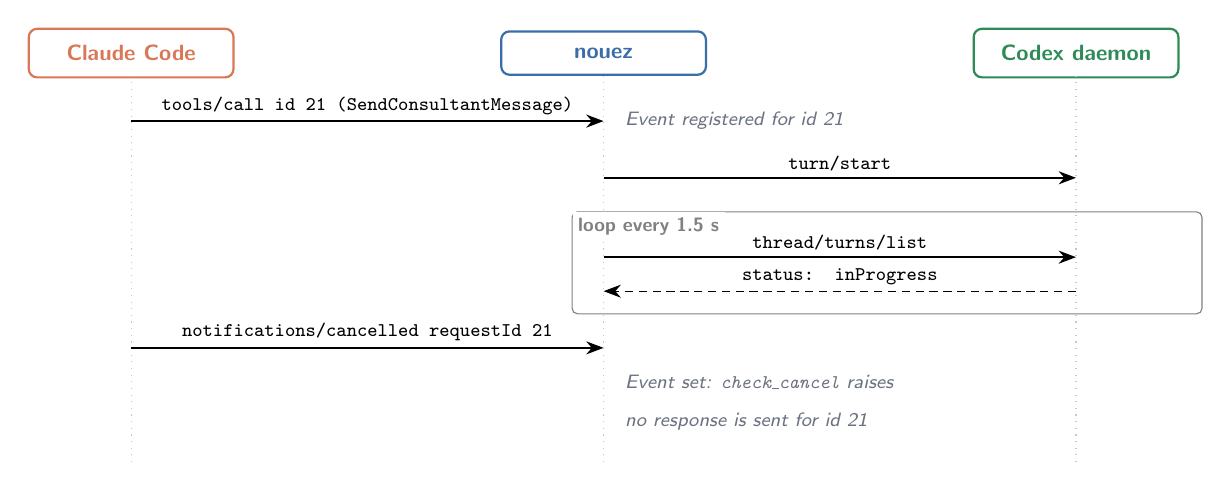
\begin{tikzpicture}[x=1cm,y=0.72cm]
  \lifelines{0/Claude Code/cc, 6/nouez/nz, 12/Codex daemon/cx}{7.2}
  \msg{1.2}{0}{6}{tools/call id 21 (SendConsultantMessage)}
  \side{1.2}{6}{Event registered for id 21}
  \msg{2.2}{6}{12}{turn/start}
  \frm{2.8}{4.6}{5.6}{13.6}{loop every 1.5 s}
  \msg{3.6}{6}{12}{thread/turns/list}
  \ret{4.2}{12}{6}{status: inProgress}
  \msg{5.2}{0}{6}{notifications/cancelled requestId 21}
  \side{5.8}{6}{Event set: \code{check\_cancel} raises}
  \side{6.5}{6}{no response is sent for id 21}
\end{tikzpicture}
\caption{Cancelling a tool call. Cancelling stops nouez from waiting; it does not stop a Codex
turn that has already started. Before delivery, the last \code{check\_cancel} runs inside the
send lock, so a cancel that arrives in time prevents the message from being sent at all.}
\end{figure}

\begin{wire}[Claude Code $\rightarrow$ nouez]
{"jsonrpc": "2.0", "method": "notifications/cancelled", "params": {"requestId": 21, "reason": "User interrupted"}}
\end{wire}

\subsection{Protocol errors}
\label{sec:errors}

Each of these except \code{-32603} is covered by \code{tests/test\_protocol.py}; the
\code{-32603} message is an example, since nothing in the tests makes \code{dispatch()} fail.
After every one of them the server keeps answering.

\begin{wire}[Line that isn't JSON: \code{\{not json} $\rightarrow$ -32700]
{"jsonrpc": "2.0", "id": null, "error": {"code": -32700, "message": "Parse error"}}
\end{wire}
\begin{wire}[Not an object (\code{[]}, \code{"hello"}), an id that isn't a string or number, or \code{"id": null} $\rightarrow$ -32600]
{"jsonrpc": "2.0", "id": null, "error": {"code": -32600, "message": "Invalid Request"}}
\end{wire}
\begin{wire}[Unknown method $\rightarrow$ -32601]
{"jsonrpc": "2.0", "id": 5, "error": {"code": -32601, "message": "Method not found: nope/nope"}}
\end{wire}
\begin{wire}[\code{"params"} that isn't an object, \code{[]} included $\rightarrow$ -32602]
{"jsonrpc": "2.0", "id": 2, "error": {"code": -32602, "message": "params must be an object."}}
\end{wire}
\begin{wire}[\code{"arguments"} that isn't an object $\rightarrow$ -32602]
{"jsonrpc": "2.0", "id": 3, "error": {"code": -32602, "message": "arguments must be an object."}}
\end{wire}
\begin{wire}[\code{"name": "Nope"} $\rightarrow$ -32602]
{"jsonrpc": "2.0", "id": 4, "error": {"code": -32602, "message": "Unknown tool: Nope"}}
\end{wire}
\begin{wire}[Unexpected failure while handling a request $\rightarrow$ -32603]
{"jsonrpc": "2.0", "id": 7, "error": {"code": -32603, "message": "Internal error: KeyError('id')"}}
\end{wire}

Argument values are checked by the tool and reported as \code{isError} results:

\begin{plain}[Tool-level validation messages]
`to` is required: the consultant name StartConsultant returned, or its thread id.
`message` is required.
`new` must be true or false, not 'yes'.
`wait` must be a number of seconds, 0 or more (0 = don't wait), or "done", not -5.
`until_done` was replaced by `wait` in nouez 0.4: pass wait="done".
`timeout_seconds` was replaced by `wait` in nouez 0.4: pass wait=<seconds>.
codex-nouez-77c2e0 is a Codex session the user opened, not a read-only consultant: it keeps the user's own permissions and may be able to edit files. Nothing was sent. Only if the user asked you to message this session, send again with allow_user_session=true; otherwise use StartConsultant.
\end{plain}
All of these are checked before anything is sent; the last one after the session is found.

% =============================================================================
\section{nouez \texorpdfstring{$\leftrightarrow$}{<->} Codex daemon}
\label{sec:codex}

\subsection{Connecting}

A tool call that gets past argument checks opens a fresh \code{CodexClient} (WatchConsultant may
open a second one) and closes it in a \code{finally} block, killing the proxy's process tree. The
connection has four steps:

\begin{figure}[H]
\centering
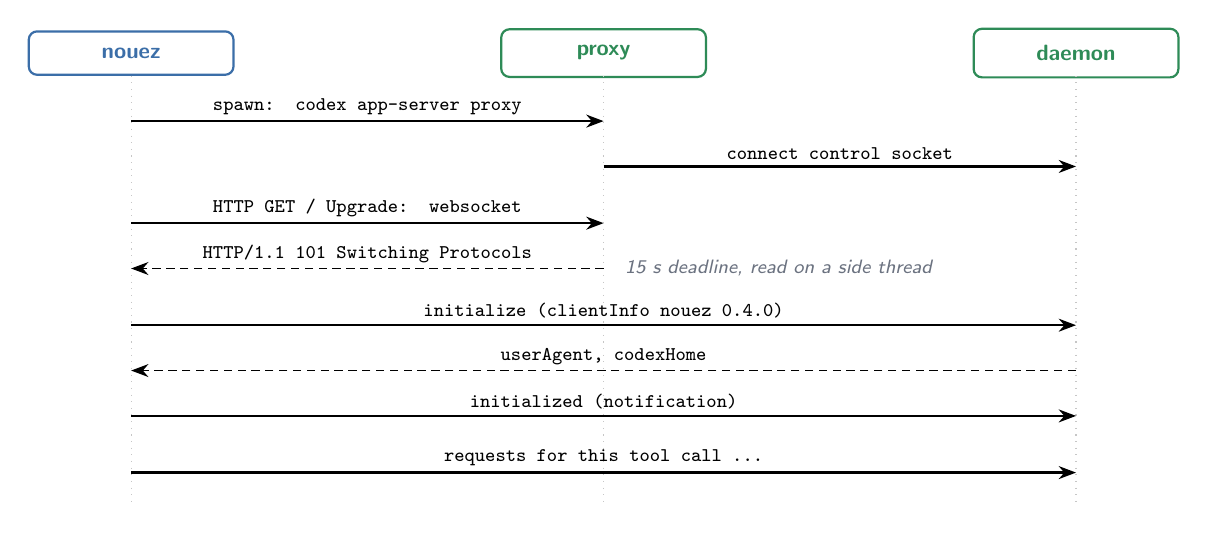
\begin{tikzpicture}[x=1cm,y=0.72cm]
  \lifelines{0/nouez/nz, 6/proxy/cx, 12/daemon/cx}{8.0}
  \msg{1.2}{0}{6}{spawn: codex app-server proxy}
  \msg{2.0}{6}{12}{connect control socket}
  \msg{3.0}{0}{6}{HTTP GET / Upgrade: websocket}
  \ret{3.8}{6}{0}{HTTP/1.1 101 Switching Protocols}
  \side{3.8}{6}{15 s deadline, read on a side thread}
  \msg{4.8}{0}{12}{initialize (clientInfo nouez 0.4.0)}
  \ret{5.6}{12}{0}{userAgent, codexHome}
  \msg{6.4}{0}{12}{initialized (notification)}
  \msg{7.4}{0}{12}{requests for this tool call ...}
\end{tikzpicture}
\caption{Opening a connection to the daemon. Bytes pass through the proxy unchanged.}
\end{figure}

\begin{plain}[nouez $\rightarrow$ proxy stdin: WebSocket upgrade]
GET / HTTP/1.1
Host: localhost
Upgrade: websocket
Connection: Upgrade
Sec-WebSocket-Key: q3Xv0m5cJ0n9aB1kL2pR8w==
Sec-WebSocket-Version: 13
\end{plain}
\begin{plain}[proxy stdout $\rightarrow$ nouez (only the status line is checked)]
HTTP/1.1 101 Switching Protocols
Upgrade: websocket
Connection: Upgrade
Sec-WebSocket-Accept: ...
\end{plain}

If the proxy closes its output before answering, nouez reports \emph{``Codex app-server daemon is
not reachable. Start it with `codex app-server daemon start`, or open a Codex session.''}; if it
says nothing within 15 seconds, \emph{``Codex app-server proxy did not respond within 15s.''}; for
any status other than 101, \emph{``WebSocket upgrade refused: <first 200 bytes of the header>''}.

\subsection{Frames}

\begin{center}\small
\begin{tabular}{@{}l l l@{}}
\toprule
\textbf{Opcode} & \textbf{Meaning} & \textbf{nouez does} \\
\midrule
\code{0x1} text, \code{0x0} continuation & a JSON message, possibly split & reassemble until FIN, then parse \\
\code{0x9} ping & keep-alive from the daemon & answer with \code{0xA} pong, same payload \\
\code{0x8} close & daemon is closing & stop reading; pending requests fail \\
\bottomrule
\end{tabular}
\end{center}

Frames nouez sends are masked, as RFC 6455 requires of clients: text frames for its messages and
pong frames for the daemon's pings. A received message over 64~MiB ends the connection. A reader
thread puts parsed messages on a queue; \code{request()} sends one message and waits up to 15
seconds for the response with the same \code{id}. Everything else the daemon sends meanwhile,
notifications and the daemon's own requests alike, is discarded. A consultant never waits on
those requests, because it was started with \code{approvalPolicy: "never"}.

\subsection{Message format}

The daemon speaks JSON-RPC without the \code{"jsonrpc"} member. Ids are integers counting from 1
on each connection.

\begin{wire}[nouez $\rightarrow$ daemon]
{"id": 1, "method": "initialize", "params": {"clientInfo": {"name": "nouez", "version": "0.4.0"}}}
\end{wire}
\begin{wire}[daemon $\rightarrow$ nouez]
{"id": 1, "result": {
  "userAgent": "codex-tui/0.162.0 (Windows 10.0.26200; x86_64) WindowsTerminal (nouez; 0.4.0)",
  "codexHome": "C:\\Users\\you\\.codex",
  "platformFamily": "windows", "platformOs": "windows"}}
\end{wire}
\begin{wire}[nouez $\rightarrow$ daemon]
{"method": "initialized"}
\end{wire}
\begin{wire}[daemon $\rightarrow$ nouez: an error response]
{"id": 7, "error": {"code": -32600, "message": "thread 01a1f3c2-... is not materialized yet"}}
\end{wire}

nouez turns an error response into \emph{``\textless method\textgreater{} failed: \textless message\textgreater''}. A few
messages mean ``this session has no history yet'' and are treated as an empty turn list rather
than a failure: \code{not materialized}, \code{missing source rollout}, \code{no rollout found},
\code{is empty}, \code{list\_turns is not supported yet}.

\subsection{Data shapes}

\begin{wire}[A thread (session), fields nouez reads; the daemon sends about 30]
{"id": "01a1f3c2-5e7b-7c41-9a0d-2b6e8c4d9f17",
 "cwd": "C:\\Users\\you\\Projects\\nouez",
 "model": "gpt-5.6-sol", "modelProvider": "openai",
 "status": {"type": "idle"},             // "idle" | "active" (+ "activeFlags") | "notLoaded" | "systemError"
 "threadSource": "nouez",                // null for sessions the user opened
 "ephemeral": false, "parentThreadId": null,
 "name": "Diff review", "updatedAt": 1791547200}
\end{wire}

The consultant's name is derived, not stored: \code{codex-} + the last folder of \code{cwd} +
\code{-} + the last six characters of the id, lower-cased: \code{codex-nouez-4d9f17}.

\begin{wire}[A turn, fields nouez reads]
{"id": "01a1f3c4-8b20-7d55-b1e3-6a9c0f2e7d31",
 "status": "completed",                  // "inProgress" | "completed" | "interrupted" | "failed"
 "error": null,                          // may be {"message": "..."} when failed or interrupted
 "items": [
   {"type": "userMessage", "content": [{"type": "text",
     "text": "[Message from Claude Code via the consultants bridge]\n\nReview this diff ..."}]},
   {"type": "agentMessage", "phase": "commentary", "text": "Reading server.py ..."},
   {"type": "agentMessage", "phase": "final_answer", "text": "Two issues. 1) ..."}]}
\end{wire}

\code{phase} is \code{"commentary"} for progress messages, \code{"final\_answer"} for the answer,
or \code{null}. For a turn that has ended, the reply is the text of all \code{agentMessage} items
with \code{phase: "final\_answer"}, or, if there are none, of the last \code{agentMessage}. For a
turn still running, nouez shows the \emph{output so far} instead: every \code{agentMessage}
after the turn's latest \code{userMessage}, whatever its phase, keeping the last 4,000
characters. A steered message adds a \code{userMessage} to the running turn, so output written
before it arrived is not shown as if it answered it. This is the snapshot from the latest poll;
nouez polls instead of following streamed events, so it may lag the session by one poll.

\subsection{Request reference}

\begin{center}\small
\begin{tabularx}{\textwidth}{@{}>{\ttfamily}l >{\raggedright\arraybackslash}X >{\raggedright\arraybackslash}X >{\raggedright\arraybackslash}p{3.2cm}@{}}
\toprule
\textrm{\textbf{Method}} & \textbf{Params nouez sends} & \textbf{Result nouez reads} & \textbf{Used by} \\
\midrule
initialize & \code{clientInfo} & \code{userAgent}, \code{codexHome} & every connection \\
thread/loaded/list & \code{\{\}} or \code{\{cursor\}} & \code{data}: ids, \code{nextCursor} & finding sessions \\
thread/read & \code{threadId} & \code{thread} & finding sessions \\
thread/list & \code{limit: 50} & \code{data}: summaries & finding unloaded consultants \\
thread/start & \code{cwd}, \code{sandbox}, \code{approvalPolicy}, \code{threadSource}, opt.\ \code{model}, \code{developerInstructions} & \code{thread} & StartConsultant \\
thread/name/set & \code{threadId}, \code{name} & -- & StartConsultant \code{title} \\
thread/resume & \code{threadId}, \code{excludeTurns: true} & -- & SendConsultantMessage \\
thread/turns/list\textsuperscript{*} & \code{threadId}, \code{limit}, \code{sortDirection: "desc"} & \code{data}: turns, with items & send, wait, reply, watch \\
turn/start & \code{threadId}, \code{input} & \code{turn.id} & send to an idle session \\
turn/steer & \code{threadId}, \code{expectedTurnId}, \code{input} & \code{turnId} (not read) & send to a busy session \\
thread/archive & \code{threadId} & -- & StopConsultant \\
\bottomrule
\end{tabularx}
\end{center}
{\small \textsuperscript{*}Codex marks \code{thread/turns/list} as experimental. nouez sends no
\code{itemsView}; the daemons it was tested with returned each turn's items, but that default is
not documented.}

\subsection{Finding a session}
\label{sec:resolve}

Every tool that takes \code{to} first lists sessions, then matches. Listing costs one request per
session, because \code{thread/list} omits \code{threadSource}:

\begin{wire}[1. Sessions loaded in the daemon (paged)]
-> {"id": 2, "method": "thread/loaded/list", "params": {}}
<- {"id": 2, "result": {"data": ["01a1f3c2-5e7b-7c41-9a0d-2b6e8c4d9f17", "01a1e8a0-..."], "nextCursor": null}}
\end{wire}
\begin{wire}[2. Read each loaded session]
-> {"id": 3, "method": "thread/read", "params": {"threadId": "01a1f3c2-5e7b-7c41-9a0d-2b6e8c4d9f17"}}
<- {"id": 3, "result": {"thread": {"id": "01a1f3c2-...", "cwd": "C:\\Users\\you\\Projects\\nouez", "threadSource": "nouez", "status": {"type": "idle"}, ...}}}
\end{wire}
\begin{wire}[3. One page of up to 50 saved sessions, to find consultants the daemon has unloaded]
-> {"id": 5, "method": "thread/list", "params": {"limit": 50}}
<- {"id": 5, "result": {"data": [{"id": "01a1d9b7-...", "status": {"type": "notLoaded"}, ...}, ...], "nextCursor": "..."}}
-> {"id": 6, "method": "thread/read", "params": {"threadId": "01a1d9b7-..."}}     // kept only if threadSource == "nouez"
\end{wire}

Only that one page is read, so a consultant unloaded and older than the 50 sessions it holds is
not listed. Then \code{to} is matched, case-insensitively: an exact name or id first; otherwise a
unique id prefix or suffix (except for \code{StopConsultant}, which accepts only exact matches);
otherwise a direct \code{thread/read} of \code{to} as a full id, which reaches older consultants.
A name keeps only the id's last six characters, so two sessions can share one; such a name is
refused, and the full id has to be used.

\begin{plain}[Matching failures (isError results)]
'codex-nouez-4d9f17' names more than one session. Use the full thread id: 01a1f3c2-5e7b-7c41-9a0d-2b6e8c4d9f17, 01a20b55-0c9e-7a13-b6f1-77e0aa4d9f17
'01a1' is ambiguous. Matches: codex-nouez-4d9f17, codex-nouez-77c2e0
No Codex session named 'codex-nouez-4d9f1'. Sessions: codex-nouez-4d9f17, codex-api-0b13aa
No Codex session named '4d9f17'. Use its exact name or full thread id. Sessions: codex-nouez-4d9f17
\end{plain}

% =============================================================================
\section{Tools, end to end}
\label{sec:tools}

Each diagram starts with a \code{tools/call} and ends with its result. ``Connect'' stands for the
handshake in Section~\ref{sec:codex}, and ``find session'' for the lookup in Section~\ref{sec:resolve}.
The example consultant is \code{codex-nouez-4d9f17}.

% -----------------------------------------------------------------------------
\subsection{StartConsultant}

Gets the consultant for a project. It reuses the most recently updated session that nouez
started in the project's git repository (outside git, in the Claude Code workspace folder that
contains \code{cwd}), and starts a new read-only one if there is none, or if \code{new: true}. It
never reuses a session the user opened, because such a session keeps the user's sandbox and
approval policy; those are only listed in the result.

\begin{figure}[H]
\centering
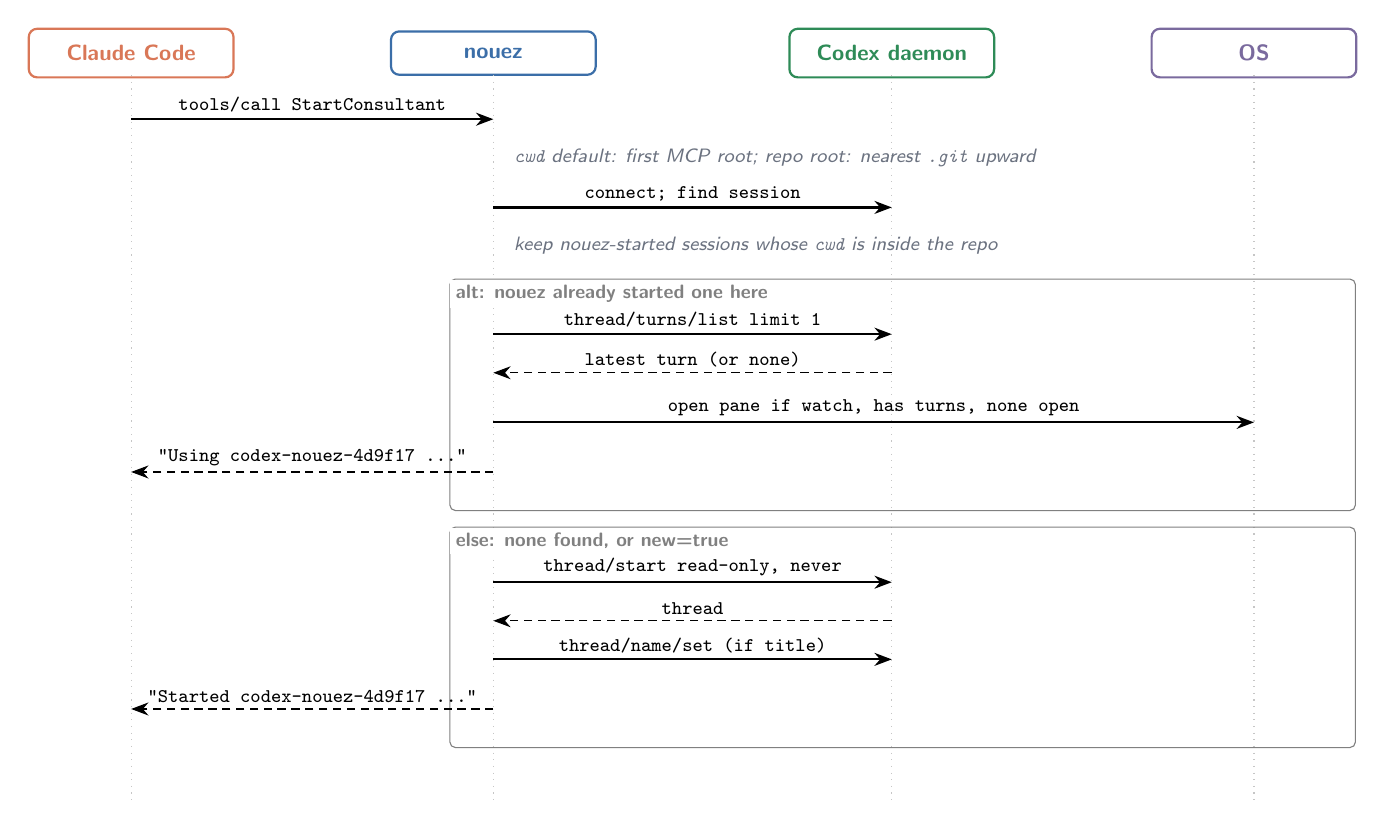
\begin{tikzpicture}[x=0.92cm,y=0.7cm]
  \lifelines{0/Claude Code/cc, 5/nouez/nz, 10.5/Codex daemon/cx, 15.5/OS/os}{13.6}
  \msg{1.2}{0}{5}{tools/call StartConsultant}
  \side{1.9}{5}{\code{cwd} default: first MCP root; repo root: nearest \code{.git} upward}
  \msg{2.8}{5}{10.5}{connect; find session}
  \side{3.5}{5}{keep nouez-started sessions whose \code{cwd} is inside the repo}
  \frm{4.1}{8.3}{4.4}{16.9}{alt: nouez already started one here}
  \msg{5.1}{5}{10.5}{thread/turns/list limit 1}
  \ret{5.8}{10.5}{5}{latest turn (or none)}
  \msg{6.7}{5}{15.5}{open pane if watch, has turns, none open}
  \ret{7.6}{5}{0}{"Using codex-nouez-4d9f17 ..."}
  \frm{8.6}{12.6}{4.4}{16.9}{else: none found, or new=true}
  \msg{9.6}{5}{10.5}{thread/start read-only, never}
  \ret{10.3}{10.5}{5}{thread}
  \msg{11.0}{5}{10.5}{thread/name/set (if title)}
  \ret{11.9}{5}{0}{"Started codex-nouez-4d9f17 ..."}
\end{tikzpicture}
\caption{StartConsultant. A new session's pane opens with its first message, because
\code{codex resume} can't show a session that has no turns yet.}
\end{figure}

\begin{wire}[Request]
{"jsonrpc": "2.0", "id": 10, "method": "tools/call", "params": {"name": "StartConsultant",
  "arguments": {"cwd": "C:\\Users\\you\\Projects\\nouez", "title": "Diff review",
                "instructions": "You are a skeptical senior reviewer. Look for bugs; don't rewrite code."}}}
\end{wire}
\begin{wire}[nouez $\rightarrow$ daemon when none exists]
{"id": 8, "method": "thread/start", "params": {
  "cwd": "C:\\Users\\you\\Projects\\nouez", "sandbox": "read-only", "approvalPolicy": "never",
  "threadSource": "nouez",
  "developerInstructions": "You are a skeptical senior reviewer. Look for bugs; don't rewrite code."}}
{"id": 9, "method": "thread/name/set", "params": {"threadId": "01a1f3c2-5e7b-7c41-9a0d-2b6e8c4d9f17", "name": "Diff review"}}
\end{wire}
\begin{plain}[Result text: started]
Started codex-nouez-4d9f17
    id: 01a1f3c2-5e7b-7c41-9a0d-2b6e8c4d9f17
    cwd: C:\Users\you\Projects\nouez
    model: gpt-5.6-sol (openai)
    sandbox: read-only
A pane showing it opens beside Claude Code when you send its first message.
Send it work with SendConsultantMessage.
\end{plain}
\begin{plain}[Result text: reused]
Using codex-nouez-4d9f17, which already works in C:\Users\you\Projects\nouez; nothing new was started.
- codex-nouez-4d9f17
    id: 01a1f3c2-5e7b-7c41-9a0d-2b6e8c4d9f17
    cwd: C:\Users\you\Projects\nouez
    model: gpt-5.6-sol (openai)
    status: idle (unloaded; reloads on the next message)
    started by: StartConsultant
    title: Diff review
Opened codex-nouez-4d9f17 in a Windows Terminal split pane.
Ignored title, instructions: they apply only to a new session (new=true).
Send it work with SendConsultantMessage.
The user's own Codex sessions in this repo were not used (they keep the user's permissions); message one only if the user asks you to:
- codex-nouez-77c2e0
    id: 01a1e8a0-1c3d-7f02-8e44-90b1d577c2e0
    ...
    started by: user
Only if the user asks for a separate consultant, call StartConsultant with new=true.
\end{plain}

The pane line is omitted with \code{watch: false}. If the session has no turns yet it reads
\emph{``A pane showing it opens beside Claude Code when you send its first message.''}, and if a
terminal already shows it, nothing is opened and the line is \emph{``... is already open in a
terminal; no new one was opened.''} The \code{watch} value of the latest StartConsultant call
also decides whether later sends open a pane. The ``Ignored'' line appears only when
\code{model}, \code{title} or \code{instructions} were passed. Other nouez sessions in the same
repository follow \emph{``Other consultants in this repo:''}, and the user-session note appears
only when there are user sessions; it is added to the ``Started'' result too.

% -----------------------------------------------------------------------------
\subsection{ListConsultants}

\begin{figure}[H]
\centering
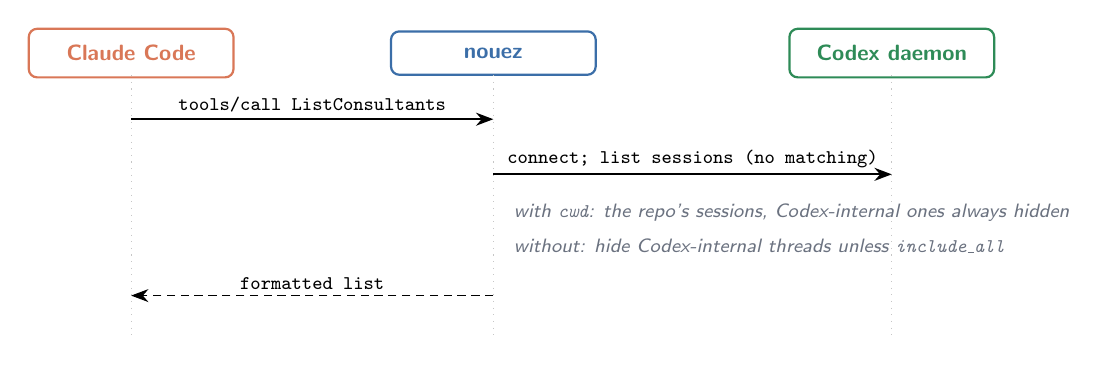
\begin{tikzpicture}[x=0.92cm,y=0.7cm]
  \lifelines{0/Claude Code/cc, 5/nouez/nz, 10.5/Codex daemon/cx}{5.2}
  \msg{1.2}{0}{5}{tools/call ListConsultants}
  \msg{2.2}{5}{10.5}{connect; list sessions (no matching)}
  \side{2.9}{5}{with \code{cwd}: the repo's sessions, Codex-internal ones always hidden}
  \side{3.5}{5}{without: hide Codex-internal threads unless \code{include\_all}}
  \ret{4.4}{5}{0}{formatted list}
\end{tikzpicture}
\caption{ListConsultants. Read-only; makes no changes. It lists the user's sessions too.}
\end{figure}

\begin{wire}[Request]
{"jsonrpc": "2.0", "id": 11, "method": "tools/call", "params": {"name": "ListConsultants",
  "arguments": {"cwd": "C:\\Users\\you\\Projects\\nouez"}}}
\end{wire}
\begin{plain}[Result text]
2 Codex session(s) in C:\Users\you\Projects\nouez:
- codex-nouez-4d9f17
    id: 01a1f3c2-5e7b-7c41-9a0d-2b6e8c4d9f17
    cwd: C:\Users\you\Projects\nouez
    model: gpt-5.6-sol (openai)
    status: busy
    started by: StartConsultant
- codex-nouez-77c2e0
    id: 01a1e8a0-1c3d-7f02-8e44-90b1d577c2e0
    cwd: C:\Users\you\Projects\nouez
    model: gpt-6-astra (openai)
    status: idle
    started by: user
\end{plain}
\begin{plain}[Result text: nothing found]
No Codex sessions in C:\Users\you\Projects\nouez. Start one with StartConsultant, or open Codex in a terminal.
\end{plain}

% -----------------------------------------------------------------------------
\subsection{SendConsultantMessage}
\label{sec:send}

The central tool. A lock per session, held only inside this nouez process, makes sure two of its
concurrent sends can't both start a turn; it does not cover other clients of the daemon, such as
the user typing in a Codex terminal. The lock is held through delivery, the check that the new
turn is listed, and opening the pane, and is released before the long wait, so a slow reply
doesn't block other senders.

\begin{figure}[H]
\centering
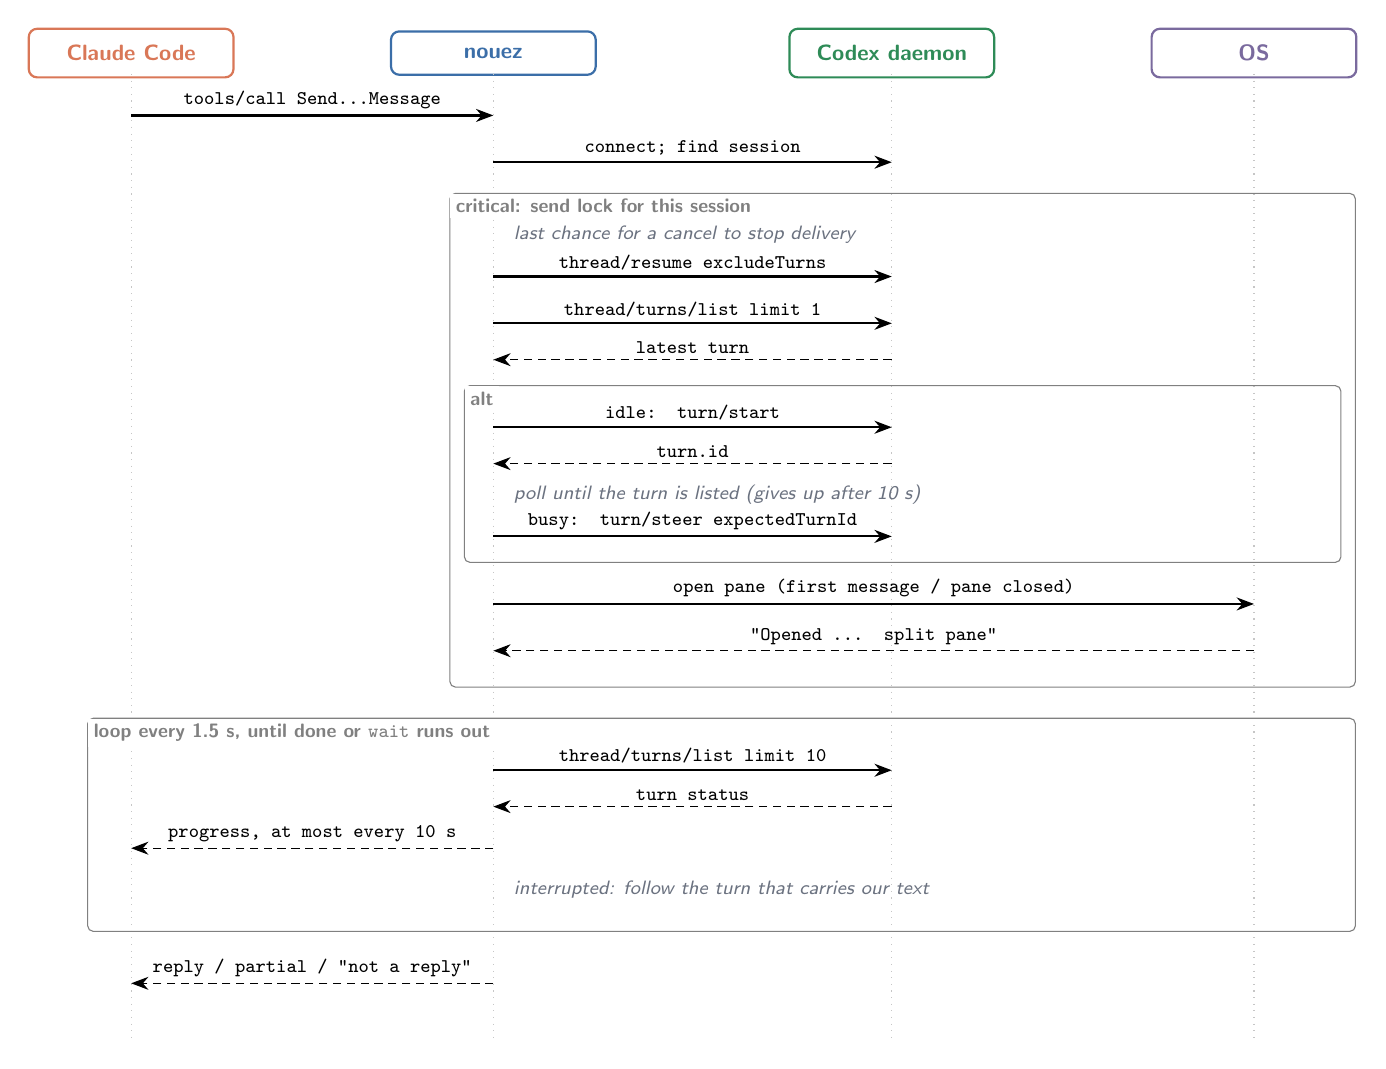
\begin{tikzpicture}[x=0.92cm,y=0.66cm]
  \lifelines{0/Claude Code/cc, 5/nouez/nz, 10.5/Codex daemon/cx, 15.5/OS/os}{19.0}
  \msg{1.2}{0}{5}{tools/call Send...Message}
  \msg{2.1}{5}{10.5}{connect; find session}
  \frm{2.7}{12.2}{4.4}{16.9}{critical: send lock for this session}
  \side{3.5}{5}{last chance for a cancel to stop delivery}
  \msg{4.3}{5}{10.5}{thread/resume excludeTurns}
  \msg{5.2}{5}{10.5}{thread/turns/list limit 1}
  \ret{5.9}{10.5}{5}{latest turn}
  \frm{6.4}{9.8}{4.6}{16.7}{alt}
  \msg{7.2}{5}{10.5}{idle: turn/start}
  \ret{7.9}{10.5}{5}{turn.id}
  \side{8.5}{5}{poll until the turn is listed (gives up after 10 s)}
  \msg{9.3}{5}{10.5}{busy: turn/steer expectedTurnId}
  \msg{10.6}{5}{15.5}{open pane (first message / pane closed)}
  \ret{11.5}{15.5}{5}{"Opened ... split pane"}
  \frm{12.8}{16.9}{-0.6}{16.9}{loop every 1.5 s, until done or \code{wait} runs out}
  \msg{13.8}{5}{10.5}{thread/turns/list limit 10}
  \ret{14.5}{10.5}{5}{turn status}
  \ret{15.3}{5}{0}{progress, at most every 10 s}
  \side{16.1}{5}{interrupted: follow the turn that carries our text}
  \ret{17.9}{5}{0}{reply / partial / "not a reply"}
\end{tikzpicture}
\caption{SendConsultantMessage with the default \code{wait} of 600 seconds. Before the lock, a
session the user opened is refused unless \code{allow\_user\_session: true}, and nothing is sent.
Progress notifications go out only if the request carried a progress token. With
\code{wait: 0} it returns after the steps inside the lock (delivery, the listing check and the pane), skipping
only the wait for the reply. The 10~s check stops polling after 10~s, but a slow
\code{thread/turns/list} request can take up to its own 15~s timeout, so it is not a hard bound.}
\end{figure}

\begin{wire}[Request]
{"jsonrpc": "2.0", "id": 14, "method": "tools/call", "params": {"name": "SendConsultantMessage",
  "arguments": {"to": "codex-nouez-4d9f17", "message": "Review this diff for bugs:\n\n```diff\n...\n```",
                "from": "Claude Code (nouez)", "wait": 600}}}
\end{wire}

Every message reaches Codex with a header naming the sender:

\begin{wire}[nouez $\rightarrow$ daemon: session idle]
{"id": 4, "method": "thread/resume", "params": {"threadId": "01a1f3c2-...", "excludeTurns": true}}
{"id": 5, "method": "thread/turns/list", "params": {"threadId": "01a1f3c2-...", "limit": 1, "sortDirection": "desc"}}
{"id": 6, "method": "turn/start", "params": {"threadId": "01a1f3c2-...", "input": [{"type": "text",
  "text": "[Message from Claude Code (nouez) via the consultants bridge]\n\nReview this diff for bugs: ..."}]}}
\end{wire}
\begin{wire}[daemon $\rightarrow$ nouez]
{"id": 6, "result": {"turn": {"id": "01a1f3c4-8b20-7d55-b1e3-6a9c0f2e7d31", ...}}}
\end{wire}
\begin{wire}[nouez $\rightarrow$ daemon: session busy, so the message steers the running turn]
{"id": 6, "method": "turn/steer", "params": {"threadId": "01a1f3c2-...",
  "expectedTurnId": "01a1f3c4-8b20-7d55-b1e3-6a9c0f2e7d31",
  "input": [{"type": "text", "text": "[Message from Claude Code via the consultants bridge]\n\nAlso check the tests."}]}}
\end{wire}
\begin{wire}[Waiting: polled every 1.5 s]
-> {"id": 9, "method": "thread/turns/list", "params": {"threadId": "01a1f3c2-...", "limit": 10, "sortDirection": "desc"}}
<- {"id": 9, "result": {"data": [{"id": "01a1f3c4-...", "status": "inProgress", "items": [...]}, ...]}}
   ...
<- {"id": 61, "result": {"data": [{"id": "01a1f3c4-...", "status": "completed", "items": [...]}, ...]}}
\end{wire}

\begin{plain}[Result text: completed]
Reply from codex-nouez-4d9f17:

Two issues. 1) route() accepts float ids but ...

(Opened codex-nouez-4d9f17 in a Windows Terminal split pane.)
\end{plain}
\begin{plain}[Result text: wait=0]
Delivered to codex-nouez-4d9f17 (started a new turn, turn 01a1f3c4-8b20-7d55-b1e3-6a9c0f2e7d31). Not waiting; read the reply with GetConsultantReply (turn_id 01a1f3c4-8b20-7d55-b1e3-6a9c0f2e7d31, wait="done").
\end{plain}
\begin{plain}[Result text: timeout (isError false; the message was delivered)]
codex-nouez-4d9f17 is still working on turn 01a1f3c4-8b20-7d55-b1e3-6a9c0f2e7d31; this is not a reply. Delivered (started a new turn), but no reply within 600s. Don't send the message again. Call GetConsultantReply with turn_id 01a1f3c4-8b20-7d55-b1e3-6a9c0f2e7d31 and wait="done" to be told when it finishes.

Output so far (a snapshot of the running turn; it may change and is not the final answer):
Reading server.py ... route() looks fine; checking dispatch next.
\end{plain}
The ``Output so far'' block is left out when the turn has written nothing since the message
arrived. If an interrupted turn carried on in a new one, the turn id given is the new one's.
\begin{plain}[Result text: waiting failed after delivery (isError true)]
Delivered to codex-nouez-4d9f17 (started a new turn, turn 01a1f3c4-8b20-7d55-b1e3-6a9c0f2e7d31), but waiting for the reply failed: thread/turns/list timed out after 15s. Don't send the message again; read the reply with GetConsultantReply (turn_id 01a1f3c4-8b20-7d55-b1e3-6a9c0f2e7d31).
\end{plain}
\begin{plain}[Result text: the turn ended without completing]
codex-nouez-4d9f17: turn 01a1f3c4-8b20-7d55-b1e3-6a9c0f2e7d31 interrupted.
Partial reply:
Reading server.py ...
If the message was folded into a later turn, read it with GetConsultantReply.
\end{plain}
\begin{plain}[Result text: reply over 60,000 characters]
Reply from codex-nouez-4d9f17:

<first 60,000 characters>

[Truncated: 18422 more characters. The full reply is saved in C:\Users\you\AppData\Local\Temp\nouez\01a1f3c4-8b20-7d55-b1e3-6a9c0f2e7d31.md.]
\end{plain}

% -----------------------------------------------------------------------------
\subsection{GetConsultantReply}

Reads a reply without sending anything. The recommended pattern for long work is to send with
\code{wait: 0} and then call this tool with the returned \code{turn\_id} and
\code{wait: "done"}. The call returns when the turn ends, when an error occurs (such as a
lost daemon connection), or after the 4-hour cap, so a client that moved it to the background is
notified when the reply is ready, up to one 1.5-second poll late. An error or the cap is not a
reply; call again.

\begin{figure}[H]
\centering
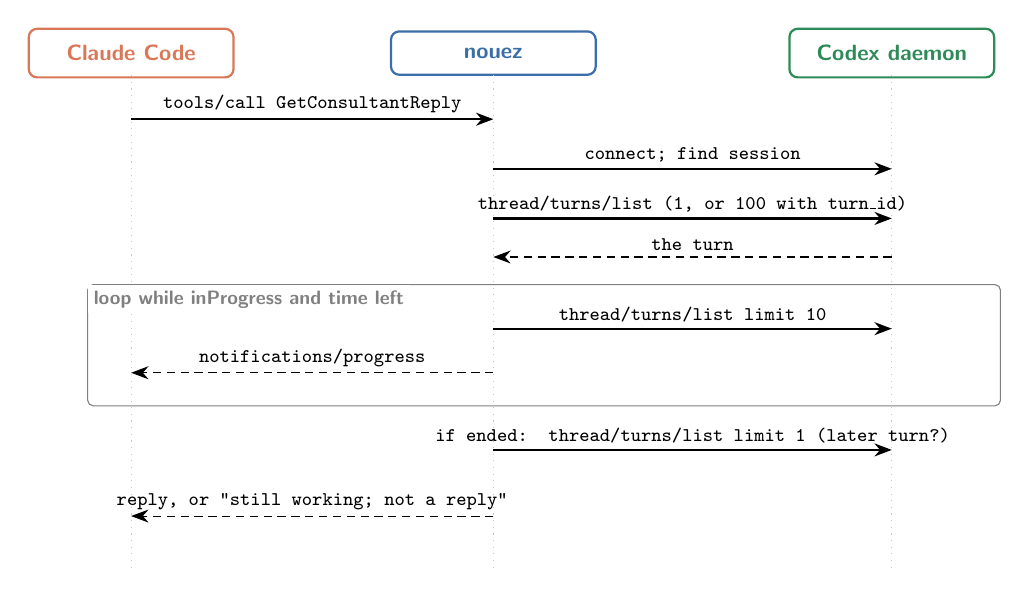
\begin{tikzpicture}[x=0.92cm,y=0.7cm]
  \lifelines{0/Claude Code/cc, 5/nouez/nz, 10.5/Codex daemon/cx}{9.4}
  \msg{1.2}{0}{5}{tools/call GetConsultantReply}
  \msg{2.1}{5}{10.5}{connect; find session}
  \msg{3.0}{5}{10.5}{thread/turns/list (1, or 100 with turn\_id)}
  \ret{3.7}{10.5}{5}{the turn}
  \frm{4.2}{6.4}{-0.6}{12.0}{loop while inProgress and time left}
  \msg{5.0}{5}{10.5}{thread/turns/list limit 10}
  \ret{5.8}{5}{0}{notifications/progress}
  \msg{7.2}{5}{10.5}{if ended: thread/turns/list limit 1 (later turn?)}
  \ret{8.4}{5}{0}{reply, or "still working; not a reply"}
\end{tikzpicture}
\caption{GetConsultantReply. \code{wait} defaults to 0: return at once. It reads user sessions too; only sending is guarded.}
\end{figure}

\begin{wire}[Request]
{"jsonrpc": "2.0", "id": 16, "method": "tools/call", "params": {"name": "GetConsultantReply",
  "arguments": {"to": "codex-nouez-4d9f17", "turn_id": "01a1f3c4-8b20-7d55-b1e3-6a9c0f2e7d31", "wait": "done"}}}
\end{wire}
\begin{plain}[Result text: variants]
Reply from codex-nouez-4d9f17:

Two issues. 1) ...

codex-nouez-4d9f17 is still working on turn 01a1f3c4-8b20-7d55-b1e3-6a9c0f2e7d31; this is not a reply. Call again with turn_id 01a1f3c4-8b20-7d55-b1e3-6a9c0f2e7d31 and wait="done" to be told when it finishes.

Output so far (a snapshot of the running turn; it may change and is not the final answer):
Reading server.py ...

codex-nouez-4d9f17 has no messages yet.

codex-nouez-4d9f17 has no turn 01a1ffff-... among its 100 most recent turns.
\end{plain}

An interrupted turn followed by a newer turn adds:
\emph{``A later turn exists (01a1f3c6-..., completed). If your message continued there, read it
by omitting turn\_id.''} nouez does not check that the later turn holds the message here; the
newer turn may be someone else's.

% -----------------------------------------------------------------------------
\subsection{WatchConsultant}

\begin{figure}[H]
\centering
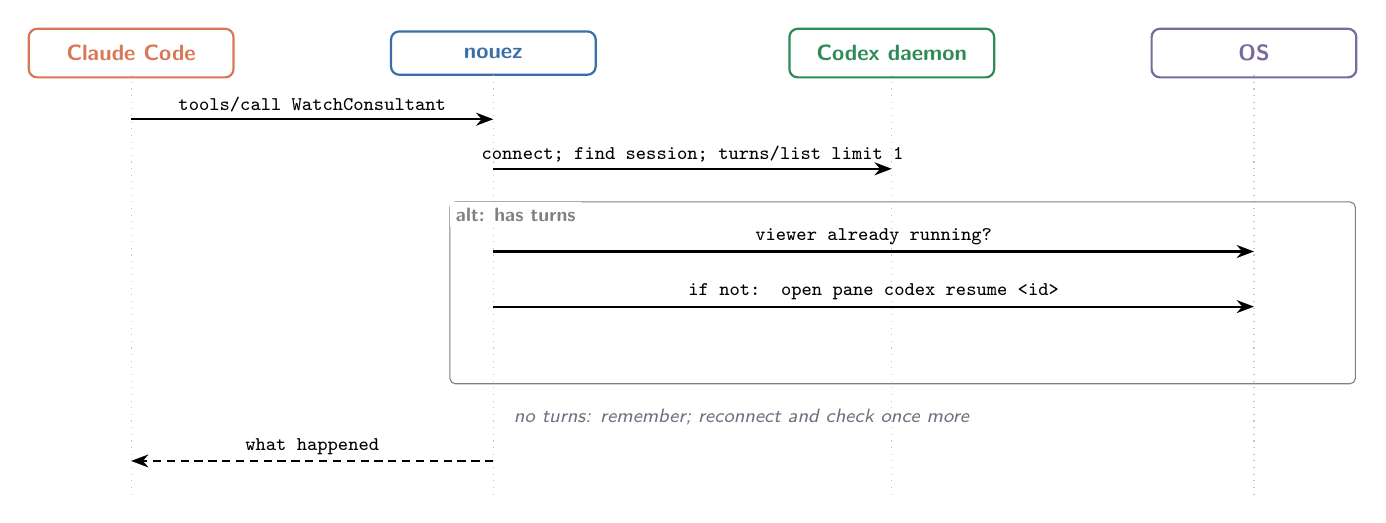
\begin{tikzpicture}[x=0.92cm,y=0.7cm]
  \lifelines{0/Claude Code/cc, 5/nouez/nz, 10.5/Codex daemon/cx, 15.5/OS/os}{8.0}
  \msg{1.2}{0}{5}{tools/call WatchConsultant}
  \msg{2.1}{5}{10.5}{connect; find session; turns/list limit 1}
  \frm{2.7}{6.0}{4.4}{16.9}{alt: has turns}
  \msg{3.6}{5}{15.5}{viewer already running?}
  \msg{4.6}{5}{15.5}{if not: open pane codex resume <id>}
  \side{6.6}{5}{no turns: remember; reconnect and check once more}
  \ret{7.4}{5}{0}{what happened}
\end{tikzpicture}
\caption{WatchConsultant. With no turns, it records the request and opens a second connection
to check again, in case a send slipped in; otherwise the next SendConsultantMessage opens the
pane. It works on the user's sessions too.}
\end{figure}

\begin{wire}[Request]
{"jsonrpc": "2.0", "id": 17, "method": "tools/call", "params": {"name": "WatchConsultant", "arguments": {"to": "codex-nouez-4d9f17"}}}
\end{wire}
\begin{plain}[Result text: variants]
Opened codex-nouez-4d9f17 in a Windows Terminal split pane.
codex-nouez-4d9f17 is already open in a terminal; no new one was opened.
codex-nouez-4d9f17 has no messages yet; a terminal window will open when you send the first one.
Opened codex-nouez-4d9f17 in Windows Terminal. Warning: the codex CLI on PATH is 0.160.1 but the daemon is 0.162.0, so the window may ask to restart the daemon. Choose Cancel (restarting interrupts running consultants) and update the codex CLI to 0.162.0.
\end{plain}

% -----------------------------------------------------------------------------
\subsection{StopConsultant}

\begin{figure}[H]
\centering
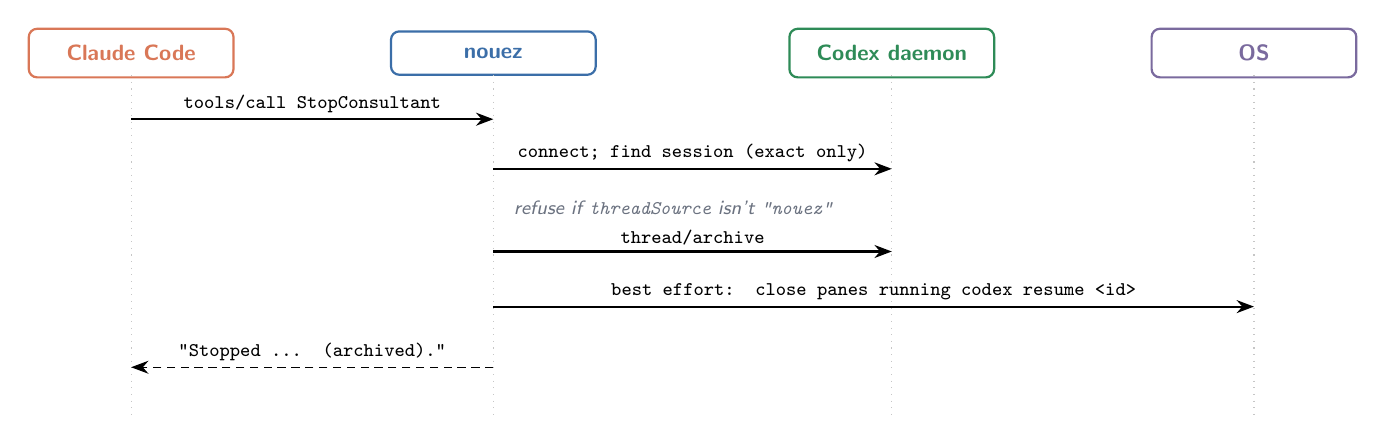
\begin{tikzpicture}[x=0.92cm,y=0.7cm]
  \lifelines{0/Claude Code/cc, 5/nouez/nz, 10.5/Codex daemon/cx, 15.5/OS/os}{6.6}
  \msg{1.2}{0}{5}{tools/call StopConsultant}
  \msg{2.1}{5}{10.5}{connect; find session (exact only)}
  \side{2.8}{5}{refuse if \code{threadSource} isn't \code{"nouez"}}
  \msg{3.6}{5}{10.5}{thread/archive}
  \msg{4.6}{5}{15.5}{best effort: close panes running codex resume <id>}
  \ret{5.7}{5}{0}{"Stopped ... (archived)."}
\end{tikzpicture}
\caption{StopConsultant. Archiving is reversible: \code{codex unarchive <id>}. Panes are found
by command line; the count in the result is how many matched, and a failed close is not
reported.}
\end{figure}

\begin{wire}[Request]
{"jsonrpc": "2.0", "id": 18, "method": "tools/call", "params": {"name": "StopConsultant", "arguments": {"to": "codex-nouez-4d9f17"}}}
\end{wire}
\begin{wire}[nouez $\rightarrow$ daemon]
{"id": 7, "method": "thread/archive", "params": {"threadId": "01a1f3c2-5e7b-7c41-9a0d-2b6e8c4d9f17"}}
\end{wire}
\begin{plain}[Result text]
Stopped codex-nouez-4d9f17 (archived). Closed 1 terminal window(s) showing it. To bring it back: codex unarchive 01a1f3c2-5e7b-7c41-9a0d-2b6e8c4d9f17, then codex resume 01a1f3c2-5e7b-7c41-9a0d-2b6e8c4d9f17.
\end{plain}
\begin{plain}[Result text: refused (isError true)]
codex-nouez-77c2e0 was not started by StartConsultant. Close it from its own terminal.
\end{plain}

% =============================================================================
\section{nouez \texorpdfstring{$\rightarrow$}{->} operating system}
\label{sec:os}

\subsection{Opening a pane}

The pane runs the daemon's own \code{codex} binary when nouez can find it, because a viewer whose
version differs from the daemon's can refuse to attach and offer to restart the shared daemon.
nouez reads the daemon's version from \code{userAgent} and looks under
\code{<codexHome>/packages/app-server-daemon/releases/<version>-*/bin/}, confirming with
\code{codex --version}.

\begin{center}\small
\begin{tabularx}{\textwidth}{@{}l >{\ttfamily\raggedright\arraybackslash}X@{}}
\toprule
\textbf{Where Claude Code runs} & \textrm{\textbf{Command nouez starts}} \\
\midrule
tmux (\code{\$TMUX} set) & tmux split-window -h -c <cwd> '<codex> resume <id>' \\
Windows Terminal (\code{\$WT\_SESSION}) & wt -w 0 split-pane -V -d <cwd> --title "Codex consultant" cmd /k <codex> resume <id> \\
Windows, \code{wt} installed & wt -w new -d <cwd> --title "Codex consultant" cmd /k <codex> resume <id> \\
Windows, no \code{wt} & cmd /c start "Codex consultant" cmd /k <codex> resume <id> \\
macOS & osascript -e 'tell application "Terminal" to do script "cd <cwd> \&\& <codex> resume <id>"' -e '... activate' \\
Linux & x-terminal-emulator -e | gnome-terminal -- | xterm -e  <codex> resume <id> \\
\bottomrule
\end{tabularx}
\end{center}

\subsection{Detecting and closing panes}

Thread ids are checked against \code{[0-9A-Za-z-]+} before they appear in any command: opening a
pane refuses a malformed id with an error, and the checks and closing skip it.

\begin{plain}[Is a viewer already running? (Windows)]
powershell -NoProfile -NonInteractive -Command
  @(Get-CimInstance Win32_Process -Filter "Name='codex.exe'" |
    Where-Object { $_.CommandLine -like '* resume 01a1f3c2-5e7b-7c41-9a0d-2b6e8c4d9f17*' }).Count
-> 1
\end{plain}
\begin{plain}[Is a viewer already running? (macOS, Linux)]
pgrep -f "codex[^ ]* resume 01a1f3c2-5e7b-7c41-9a0d-2b6e8c4d9f17"
\end{plain}
\begin{plain}[Closing on StopConsultant (Windows), abridged: find the cmd windows nouez opened, with their children]
powershell ... Get-CimInstance Win32_Process -Filter "Name='cmd.exe'" |
  Where-Object { $_.CommandLine -like '*/k *codex* resume 01a1f3c2-...' } | ForEach-Object { "$p $k" }
-> 18244 20112
taskkill /PID 20112 /T /F            (codex inside the pane)
TerminateProcess(18244, exit code 0) (cmd; a clean exit lets Windows Terminal close the pane)
\end{plain}
\begin{plain}[Closing on StopConsultant (macOS, Linux)]
pkill -f "codex[^ ]* resume 01a1f3c2-5e7b-7c41-9a0d-2b6e8c4d9f17"
\end{plain}

The last two lines are what nouez does, not commands it runs: \code{taskkill} is run per child,
and the cmd process is ended through the Win32 \code{TerminateProcess} call.

Each check and close command has a timeout (20~s; 10~s for \code{codex --version}). When it
fires, nouez stops reading the command's pipes, because on Windows a grandchild process can keep
a pipe open forever, and kills the process: the whole tree on Windows (\code{taskkill /T}), only
the direct process elsewhere. The pane itself is started without waiting, so it has no timeout.

% =============================================================================
\section{Limits and constants}

\begin{center}\small
\begin{tabular}{@{}l l l@{}}
\toprule
\textbf{Constant} & \textbf{Value} & \textbf{Meaning} \\
\midrule
\code{PROTOCOL\_VERSIONS} & 2025-11-25, 2025-06-18, 2025-03-26 & MCP versions answered \\
\code{SANDBOX} & \code{read-only} & sandbox of every started consultant \\
\code{BRIDGE\_SOURCE} & \code{nouez} & \code{threadSource} tag on started sessions \\
\code{POLL\_SECONDS} & 1.5 s & turn polling interval \\
\code{PROGRESS\_SECONDS} & 10 s & least time between progress notifications \\
\code{MAX\_WAIT\_SECONDS} & 4 h & cap on polling for a turn, \code{wait: "done"} included \\
\code{MAX\_REPLY\_CHARS} & 60,000 & longer replies are cut and saved to a file \\
\code{PARTIAL\_CHARS} & 4,000 & output so far shown for a running turn (the end) \\
\code{RECENT\_SAVED\_THREADS} & 50 & saved sessions checked for unloaded consultants \\
\code{REPLY\_LOOKBACK} & 100 & turns searched for a \code{turn\_id} \\
\code{MAX\_FRAME\_BYTES} & 64 MiB & largest WebSocket message accepted \\
Daemon request timeout & 15 s & per Codex request and for the handshake \\
\code{roots/list} timeout & 5 s & then nouez assumes no roots \\
Default \code{wait} & 600 s / 0 s & SendConsultantMessage / GetConsultantReply \\
\bottomrule
\end{tabular}
\end{center}

\end{document}
